\section{Framework}
%\BF{workflow figure to show the framework}
%\begin{multicols}{2}
%\begin{figure*}
%\centering
%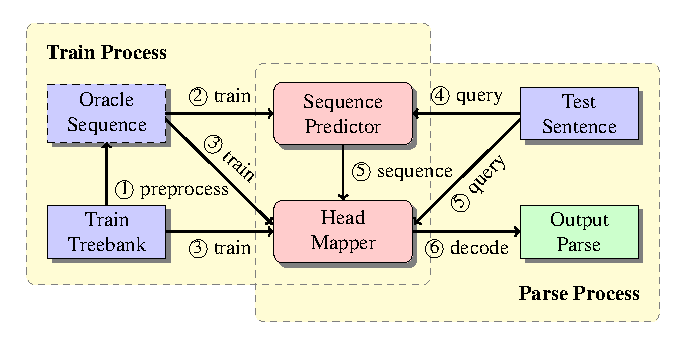
\includegraphics[width=2\columnwidth]{sysoverviewgrapheps.eps}
%\caption{Framework wrokflow} \label{fig:workflow}
%\end{figure*}
%\end{multicols}
%\KZ{In the framework, say ``Output Parse'' instead of ``Output File.''}
The general architecture of the our parser is shown in \figref{fig:workflow}
and is divided into training phase and parsing phase.
%We take training treebank as input, which carries the
%essential information (we only use FORM and POSTAG) and
%gold dependency parses.

\begin{figure}[th]
\centering
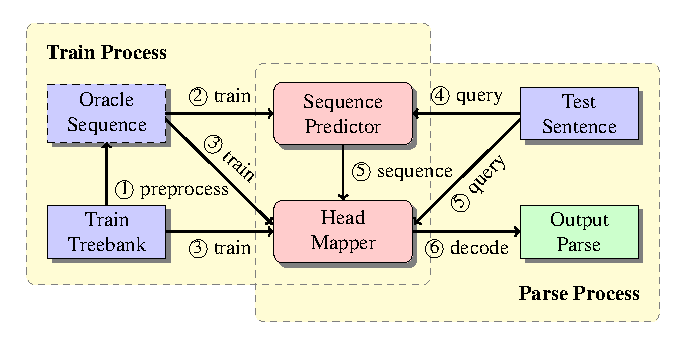
\epsfig{file=sysoverviewgrapheps.eps, width=\columnwidth}
\caption{Sequence Based Parser Framework}
\label{fig:workflow}
\end{figure}

{\bf Training:} The preprocessing step generates oracle sequences
from the gold standard parse trees. Only the word forms and the POS tags 
in these parse trees are used. Here, we assume that a child node is
easier to process than its parent node and it is supposed to be attached
before its parent. \footnote{By this rule, multiple gold sequences
can be generated from one dependency tree. In this paper, when a parent node
has multiple children, we generate the sequence by a left-to-right order.}
%\KZ{Which one do we use or do we use all of them?}
%\footnote{
%For example, a bottom-up, breadth-first traversal of the gold parse tree or oracle transition
%process order from Malt Parser are both gold sequences.}
%and further discussion is deferred to Section 4.
%\TJ{maybe they will ask which one is the best; needs some explanations here}
We then train respectively a graph-based head mapper (a.k.a. decoder)
from the gold sequences and the gold parses, and a sequence predictor
from the gold sequences.

{\bf Parsing:} Given an input sentence, the sequence predictor
outputs a feasible decoding sequence, which is a permutation of
the words in the input. For each word in this sequence,
the head mapper returns its best head word according to a scoring function
while employing a cycle detection mechanism.
The process continues until all words in the sentence have found their
heads.
%(except manually introduce ROOT node in dependency parsing).
%For a sentence with $N$ words, the final result consists of ($N+1$) nodes
%and constructed $N$ arcs.
The procedure guarantees to produce a tree structure eventually.
\cut{
We implemented a simple version of this framework,
%and released the source code as well as the evaluation data\footnote{\urlstyle{same}\url{https://github.com/littlebeanfang/BeanParser}}.
%To reproduce the experiments refered in this paper, all our data and related commands are offered in the compressed file.
%\BF{add the data download source}
%\KZ{Besides the open-source system, create an online demo using default model
%and allow users to type in
%a sentence to have it parsed.}
and built an online demo\footnote{\urlstyle{same}\url{http://202.120.38.146/BeanParser}} to show parses of eight languages with the model
trained in our experiment.}

In the current implementation, we generate the decoding sequence by
{\em stackproj} algorithm~\cite{nivre2009non} in
malt parser and scorer-based greedy head mapper.
%\KZ{Consider rephrase this sentence.
%What does graph-based head mapper have to do with sequence?}
%The training and testing data are both in
%CoNLL format~\footnote{http://ilk.uvt.nl/conll/}.

